\section{Introduction}
% Just a first sketch:
This Bachelor Thesis is about writing a fast and interactive 3D visualization environment for scientific computing. 
The focus is on usability, applied to all the different interfaces, ranging from abstract API interfaces to graphical user interfaces. 
The ultimate goal is to make scientific computing more accessible to the user.
As \ac{GUI} elements and editable text fields are supplied, one can also write and execute scripts.
Using these widgets, all bound variables can be visualized and some of them can be edited interactively. 
This can be used as a basis for interactive programming or visual debugging, further helping the user to understand his algorithms.

The introduction is structured in the following way.
First, an introduction to the general field of research and its challenges is given. 
From these challenges, the problems relevant to this thesis will be extracted.
Finally this chapter will conclude with a solution to the problem, how to measure the success and give an outlook on the structure of the entire Bachelor Thesis.


\subsection{Scientific Computing}
Scientific computing is the area of computing, that evolves around all kind of scientific research.
It is a very broad field involving a lot of different challenges. In some areas like particle physics, the problems are computationally so demanding, that they can only be solved with the help of super computers. In other areas like robotics, it is important to be fast, while running on embedded systems with small resources. In mathematics, speed does not need to be important, but it can be that the algorithm in itself is very difficult to comprehend. So the more comprehendable it can be written down in a programming language, the easier it will be to actually implement the algorithm.
Above all, programming itself is often secondary to the research goal.
This means, that it can be expected that the researcher just has rudimentary programming skills and that he does want to put as little time as possible into solving programming problems.
So things like manual memory management and difficult design patterns with a lot of boilerplates are to be avoided in scientific computing.
This has lead to the rise of programming languages and tools specifically tailored to scientific computing.
The most prominent examples include Mathematica, R and Matlab. 
They all aim to provide simple syntax for linear algebra stastical code, while taking away programatically difficult tasks like memory management. Also, they come with a rich standard library, which means most research can be done without loading any addtional module, which makes them great tools for rapid prototyping.
At the current state, the speed of these languages suffer from the high level of abstraction. In order to cater to scientific research which is in need of highly performant code, a lot of the core is written in another language like C/C++ and Fortran.
This leads us straight to the contributation of this thesis.

\subsection{Contribution}
The contribution of this thesis is an interactive visualization library tied to a fast scientific computing language, while entirely written in the same language.

\subsection{Field of Research and Problem}

\vspace{1em}
\begin{minipage}{\linewidth}
    \centering
    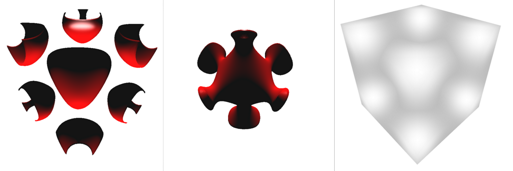
\includegraphics[width=0.7\linewidth]{graphics/surfaces.png}
    \captionof{figure}[Volume Visualization]{different visualizations of $f(x,y,z)=\sin(\frac{x}{15})+\sin(\frac{y}{15})+\sin(\frac{z}{15})$, visualized with Romeo. From left to right: Isosurface with isovalue=0.76, Isosurface with isovalue=0.37, maximum value projection}
    \label{fig:volume}
\end{minipage}
\vspace{1em}

%Scientific computing: visual debugging, interactive programming, high performance
%First rough sketch:
The general research field is making the capabilities of computers more accessible and understandable.
This is a very broad definition and there are many different ways of making it easier to use a computer. 
One of the first big steps was to move from coding in binary to assembly. 
Many more steps have followed, for example introducing graphical user interfaces, novel input devices like the mouse, understandable visualizations and so forth.
All these advances have made computers usable even for people who don't have an education in computer science.
In this bachelor thesis the field is scientific computing, which still has quite a lot of barriers for novel users.
Scientific computing is usually about implementing mathematical equations, complex algorithms and manipulating and analyzing data.
As it is difficult to offer easy to use graphical interfaces for this kind of work, most research is done in some specialized, high-level scientific computing language. As most high-level languages are relatively slow, but for a lot of algorithms state of the art performance is required, this has led to a dual system. Prototyping in a high-level language, and then redoing the work in a fast low-level language.
That this is not the perfect work flow is immediately visible, and a lot of research has been put into making high-level languages faster.
These efforts slowly pay off and there is a whole new range of languages, that claim to be easy to work with while being as fast as it can get.
This is a relatively recent trend and hasn't fully arrived in scientific computing yet, as most languages still have their core implemented in another fast language, which makes it hard to extend them for non professional users.
This is especially true for high performance visualization libraries, which mostly use C++ at their performance critical core.
To leverage the extensibility of these libraries, this bachelor thesis implements a visualization library in a fast high level language.
Visualizations where chosen as they are a crucial building blocks for many fields in scientific computing.

Consider the following function $f(x,y,z)=\sin(\frac{x}{15})+\sin(\frac{y}{15})+\sin(\frac{z}{15})$, which describes a 3D volume mathematically. 
This is a simple function, which is already not that easy to interpret. In figure \ref{fig:volume}, you can see different visualizations of f. 
Especially for more complex functions, visualizing might be the only way to get a deeper understanding of the values that a formula or algorithm produces.
This deeper understanding is crucial for identifying problems in the underlying math, or extending the algorithm.
Additionally, widgets and simple \ac{GUI}s are indispensable, giving scientist an easy way to interact with their data and algorithms.
This helps to further understand the dynamics of the data and quickly spot mistakes.

In summary, the software in this thesis (Romeo) focuses on research which involves writing short scripts, while playing around with some parameters and visualizing the results. 
An example would be a material researcher, who is investigating different 3D shapes and materials and their reaction to pressure.
The researcher would need to read in the 3D object he wants to analyze, have an easy way to tweak the material parameters and it would be preferable to get instant feedback on how the pressure waves propagate through the object.


\subsection{Outlook}
%Structure of BA and a few worts on the results 


